\documentclass{article}[18pt]
\usepackage{../../../../format}
\lhead{A Level Maths - FP2}
\usepackage{tabularx}
\begin{document}
\begin{center}
\underline{\huge FP2 Cheat Sheet}
\end{center}
\section{Inequalities}
We can build upon our previous algebraic skills in order to solve more complex inequalities\\
Remember:
\begin{itemize}
\item Don't multiply anything that could be negative - use "squared" things
\item Try to avoid fully expanding where possible
\item Find the critical values (f(x)=0)
\item Sketch the graph to solve
\end{itemize}
\section{Series}
Summations can sometimes be simplified using the method of differences\\
\\
This involves a summation where one term is subtracted from another, often gained from partial fractions. The terms in the middle of the series will then cancel with each other, leaving the summation just the terms at the beginning at the end, by summing these a simpler form can be gained.
\section{Further complex numbers}
Remember that complex fractions can be rationalised by multiplying the top and bottom by the complex conjugate
\subsection{Converting between forms}
When converting from $x+iy$ to a form in r and $\theta$, take the angle from the positive $x$ axis
\subsection{Multiplying and dividing complex numbers}
It is easiest to use the exponential form, then convert if needed
\subsubsection{Multiplying}
$$Z_1Z_2=r_1e^{i\theta_1}\times r_2e^{i\theta_2}=r_1r_2e^{i(\theta_1+\theta_2)}$$
\subsubsection{Dividing}
$$\frac{Z_1}{Z_2}=r_1e^{i\theta_1}\div r_2e^{i\theta_2}=\frac{r+1}{r+2} e^{i(\theta_1-\theta_2)}$$
\subsection{De Moivre's theorem}
This is given on the data sheet and has multiple applications
\subsubsection{Roots of unity}
When solving $z^a=r(\cos(\theta)+i\sin(\theta))$ type questions, remember to first rewrite as:
$$z^a=r(\cos(\theta+2k\pi)+i\sin(\theta+2k\pi))$$
\subsubsection{Powers of cos/sin$\rightarrow$Multiples of $\theta$}
If $z=\cos\theta+i\sin\theta$
$$z+\frac{1}{z}=2\cos\theta$$
$$z-\frac{1}{z}=2i\sin\theta$$
$$z^n+\frac{1}{z^n}=2\cos n\theta$$
$$z^n-\frac{1}{z^n}=2i\sin n\theta$$
These can be calculated by using DMs theorem to find $z^{-1} =\frac{1}{z}$ then adding or subtracting
\subsubsection{Multiples of $\theta\rightarrow$ Powers of cos/sin}
Whatever the multiple of $\theta$ is, raise $(\cos\theta+i\sin\theta)$ to that power. Use De Moivre's theorem to express this in multiples of $\theta$, and use binomial expansion to express it in terms of powers of $\theta$. Equate the real/imaginary parts, depending on whether it is cos or sin to simplify.

\subsection{Loci on the complex plane}
{\renewcommand{\arraystretch}{2}
\begin{tabularx}{\textwidth}{|X|X|}
\hline
Equation&Description\\
\hline
{\Large$|z-z_1|=r$}&A circle centre $(x_1,y_1)$ with a radius r\\
\hline
{\Large$|z-z_1|=|z-z_2|$}&A perpendicular bisector of the line segment joining points $z_1$ and $z_2$\\
\hline
{\Large$|z-z_1|=\lambda|z-z_2|$}&A circle, the equation of which is best found algebraically\\
\hline
{\Large$\arg(z-z_1)=\theta$}&The half line from a fixed point $z_1$, making an angle $\theta$ with the positive real axis\\
\hline
{\Large$\arg(\frac{z-z_1}{z-z_2})=\theta$}&An arc between the points $z_1$ and $z_2$ where the angle the lines from $z_1$ and $z_2$ to any point on the arc is $\theta$\\
\hline
\end{tabularx}}
\subsubsection{Cartesian equations of loci}
Method for modulus questions:
\begin{itemize}
\item Replace $z$ with $x+iy$
\item Group real and imaginary parts if needed
\item Use $|x+iy|=\sqrt{x^2+y^2}$
\item Complete the square if you know you're going to get a circle
\end{itemize}
Argument equations:
For lines, check by looking at the graph, but use
$$\frac{Im}{R_e}=\tan\theta$$
Remove the i from the imaginary part when putting it in the fraction, but remember that x and y are supposed to stay\\
For circles, find the centre and radius, and use this to form the equation, though remember to include $y>0$, where often necessary as it is an arc from the x axis
\subsection{Translations}
\begin{itemize}
\item $w=z+a+ib$ represents a translation with translation vector $\begin{pmatrix}
a\\b
\end{pmatrix}$
\item $w=kz$ represents an enlargement with scale factor $k$ centre $(0,0)$
\item $w=kz+a+ib$ represents an enlargement scale factor $k$ centre $(0,0)$ followed by a translation with translation vector $\begin{pmatrix}
a\\b
\end{pmatrix}$
\item $w=z^2$ multiply a shape by itself, for example a circle of radius 4 would go to radius 16
\end{itemize}

\section{First order differential equations}
\subsection{Solving first order DE using an integrating factor}
Solving $\dfrac{dy}{dx}+P(x)y=Q(x)$\\
\\
IF(Integrating factor) is found by finding $\mathlarger{e^{\int p(x) \ dx}}$ And multiplying the DE by the IF.\\
\\
This will result in the DE being in the form:
$$f(x)\frac{dy}{dx}+f'(x)y$$
This form can then be shortened by integrating:
$$\int f'(x)g(x)+f(x)g'(x) dx=f(x)g(x)+c$$
Integrate both sides then simplify
\section{Second order differential equations}
{\renewcommand{\arraystretch}{2}
\begin{tabularx}{\textwidth}{|X|X|X|}
\hline
\textbf{Solution to auxiliary equation}&\textbf{General solution}&\textbf{Trig general solution}\\
\hline
Two real roots $b^2>4ac$&$Ae^{\alpha x}+Be^{\beta x}$&\\
\hline
One real root $b^2=4ac$&$(A+bx)e^{\alpha x}$&\\
\hline
Imaginary only root $b^2<4ac$&$Ae^{\alpha x}+Be^{-\alpha x}$&
$p\cos\alpha x+q\sin\alpha x$
\\
\hline
Complex root $b^2<4ac$&$Ae^{(\beta+\alpha i)x}+Be^{(\beta-\alpha i)x}$&
$e^{\beta x}(P\cos\alpha x+Q\sin\alpha x)$
\\
\hline
\end{tabularx}}
P=A+B\\
Q=i(A+B)
\subsection{Second ODE=f(x)}
\subsubsection{Standard forms of f(x)}
$f(x)=\lambda$\\
$f(x)=\lambda+\mu x$\\
$f(x)=\lambda+\mu x+\nu x^2$\\
$f(x)=ke^{px}$\\
$f(x)=m\cos\omega x$\\
$f(x)=m\sin\omega x$\\
$f(x)=m\cos\omega x\pm n\sin\omega x$
\\
To solve these find $\frac{dy}{dx}$ and $\frac{d^2y}{dx^2}$ and substitute them into the Second ODE, solving for the unknowns, then add them to the general solution.\\
\\
If there is a clash of terms between the CF and PI, then an alternate PI will be given to you. If in doubt, multiply the standard form through by x, but this will not always work.
\subsection{Boundary conditions}
If boundary conditions are given to you, the values of the unknowns can be found. Substitute the boundary conditions in and rearrange to find unknowns.
\newpage
\subsection{Substitution}
Transformations can be used to simplify differential equations, leaving $\frac{d^2y}{dx^2}$ with no coefficient.\\
Method:\\
\textcolor{red}{\large Find $\frac{dy}{dx}$ in terms of $\frac{dy}{du}$}
$$x=e^u \quad \frac{dx}{du}=e^u \quad \frac{du}{dx}=e^{-u} \quad 
\frac{dy}{dx}=\frac{dy}{du}\times\frac{du}{dx}=\mathbf{e^{-u}\frac{dy}{du}}
$$
\textcolor{red}{\large Find $\frac{d^2y}{dx^2}$ in terms of $\frac{d^2y}{du^2}$ and $\frac{dy}{du}$}\\
\textcolor{red}{Find $\frac{dy}{du}\Big(\frac{dy}{dx}\Big)$ by applying the product rule}
$$\frac{dy}{du}\Big(\frac{dy}{dx}\Big)=-e^{-u}\frac{dy}{du}+e^{-u}\frac{d^2y}{du^2}$$
\textcolor{red}{Multiply through by $\frac{du}{dx}$ to find the value of $\frac{d^2y}{dx^2}$}
$$\frac{d^2y}{dx^2}=\frac{dy}{du}\Big(\frac{dy}{dx}\Big)\times\frac{du}{dx}$$
$$\frac{d^2y}{dx^2}=e^{-u}\Big(-e^{-u}\frac{dy}{du}+e^{-u}\frac{d^2y}{du^2}\Big)$$
$$\frac{d^2y}{dx^2}=\mathbf{e^{-2u}\Big(-\frac{dy}{du}+\frac{d^2y}{du^2}\Big)}$$
\textcolor{red}{Then substitute the values for x,$\frac{dy}{dx}$, and $\frac{d^2y}{dx^2}$ into the original equation to simplify it}

\section{Maclaurin and Taylor Series}
Use the formulas on the data sheet, remember than things like lns can be simplified if they look impossible to solve.
\subsection{Solving differential equations using the Taylor expansion}
From the differential equation, calculate the values of $\frac{dy}{dx}$, $\frac{d^2y}{dx^2}$ etc up to whatever is needed.\\
Then substitute those values into the Taylor series to solve the differential equation
\section{Polar Coordinates}
\begin{tabularx}{\textwidth}{|X|X|}
\hline
Equation&Description\\
\hline
$r=a$&A circle, centre (0,0) with a radius of a\\
\hline
$\theta=\alpha$&A half line starting from (0,0) making an angle $\alpha$ with the initial line\\
\hline
$r=a\theta$&A spiral starting at the origin\\
\hline
$r=a(1+\cos\theta)$&A cardioid with x intercept a\\
\hline
$r^2=a^2\cos2\theta$&An infinity symbol with x intercept of a\\
\hline
$r^2=a^2\sin2\theta$&Infinity symbol rotated by $\frac{\pi}{4}$\\
\hline
$r=a\sin3\theta$&A windmill with 3 blades\\
\hline
\end{tabularx}
\newpage
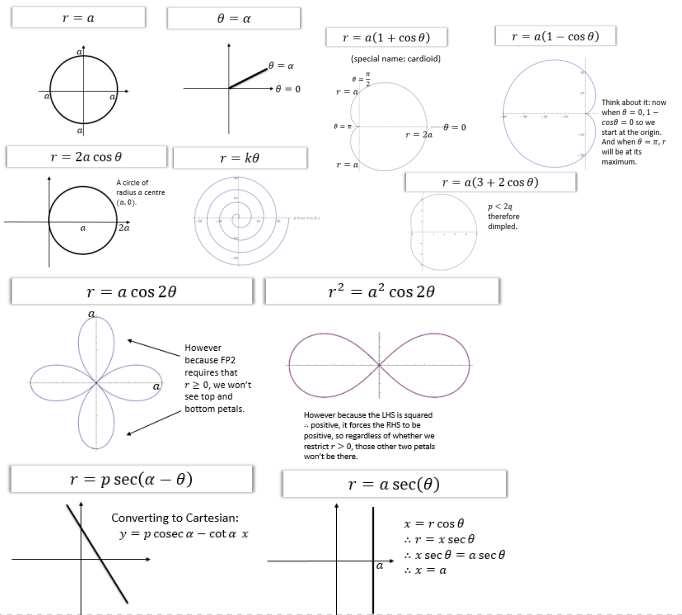
\includegraphics[width=18cm]{polar.png}\\
For $r=p\sec(\alpha-\theta)$ to solve it, divide both sides by $\sec(\alpha-\theta)$, then use the cos addition formula and simplify.
\subsection{Integration}
$$\textrm{Area}=\frac{1}{2}\int_\alpha^\beta r^2 \ d\theta$$
The area of the sector is bounded by the half lines $\theta=\alpha$ and $\theta=\beta$
\subsection{Differentiation}
To find tangents parallel and perpendicular to the initial line:\\
\\
Parallel: $\frac{dy}{d\theta}=0$\\
Perpendicular: $\frac{dx}{d\theta}=0$






\end{document}




